% 图 6.8 二维伊辛模型（按原书 117 页样式：+/− 字符栅格 9x9，点线勾出缺陷边界）
% 缺陷布局照原书：r3:c6,7  r4:c5,6,7  r5:c5,6  r6:c5,6  r7:c5
\documentclass[tikz,border=5pt]{standalone}
\usepackage{amsmath}
\usepackage{fontspec}
\setmainfont{Times New Roman}
\begin{document}
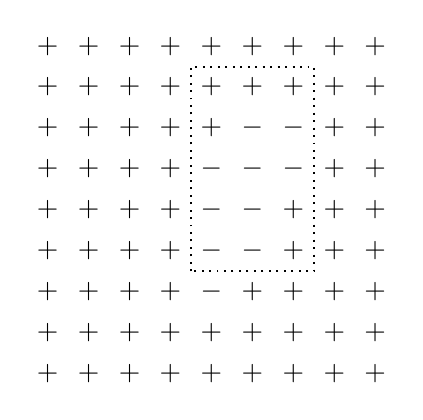
\begin{tikzpicture}
\def\s{0.52}
% ---- 点线边界：包住全部 − 自旋（照原书矩形框） ----
\draw[dotted,line width=0.7pt]
  ({4.5*\s},{2.5*\s}) rectangle ({7.5*\s},{7.5*\s});
% ---- 9x9 栅格：+ 上自旋，− 下自旋 ----
\foreach \r in {1,...,9}{
  \foreach \c in {1,...,9}{
    % 判定是否 − 格点
    \def\isminus{0}
    \ifnum\r=3\ifnum\c=6\def\isminus{1}\fi\ifnum\c=7\def\isminus{1}\fi\fi
    \ifnum\r=4\ifnum\c=5\def\isminus{1}\fi\ifnum\c=6\def\isminus{1}\fi\ifnum\c=7\def\isminus{1}\fi\fi
    \ifnum\r=5\ifnum\c=5\def\isminus{1}\fi\ifnum\c=6\def\isminus{1}\fi\fi
    \ifnum\r=6\ifnum\c=5\def\isminus{1}\fi\ifnum\c=6\def\isminus{1}\fi\fi
    \ifnum\r=7\ifnum\c=5\def\isminus{1}\fi\fi
    \node at ({\c*\s},{(9-\r)*\s}) {%
      \ifnum\isminus=1 $-$\else $+$\fi};
  }
}
\end{tikzpicture}
\end{document}
